\documentclass[12pt,oneside]{memoir}

\usepackage{amsmath}
\usepackage{amssymb}
\usepackage{amsthm}
\usepackage{algorithm}
\usepackage{algpseudocode}
\usepackage{bm}
\usepackage{color}
\usepackage{hyperref}
\usepackage[htt]{hyphenat}
\usepackage{listings}
\usepackage{mathrsfs}
\usepackage{natbib}
\usepackage{subcaption}
\usepackage{tikz}
\usepackage{todonotes}

% change the default typewriter font to inconsolata
%\usepackage{inconsolata}

% Using Courier font
\renewcommand{\ttdefault}{pcr}

% tiny
% scriptsize
% footnotesize
% small
% normalsize
% large
% Large
% LARGE
% huge
% Huge




% draw UML diagrams
\usepackage[simplified]{pgf-umlcd}
% new environment for UML diagrams
\newenvironment{myuml}%
{\begin{tikzpicture}[font=\ttfamily\scriptsize]}%
{\end{tikzpicture}}

% Number parts, chapters, sections, subsections and subsubsections
\setcounter{secnumdepth}{3}
% Put parts, chapters, sections, subsections and subsubsections in the
% table of contents
\setcounter{tocdepth}{1}

% logical entity modeled in supply chain
\newcommand{\entity}[1]{\textsc{#1}}

% name of Java class
%\usepackage{url}
%\DeclareUrlCommand\code{\urlstyle{tt}}
\newcommand{\code}[1]{{\scriptsize\texttt{#1}}}


\newcommand{\mytodo}[1]{\todo[inline]{#1}}

% a mod b
\newcommand{\amodb}[2]{#1\,\bmod\,#2}


\newtheorem{definition}{Definition}


\listfiles




%\usepackage{showkeys}
% wrap labels from showkeys package
%\renewcommand*\showkeyslabelformat[1]{%
%\fbox{\parbox[t]{\marginparwidth}{\raggedright\normalfont\small\ttfamily#1}}}



% all information up to the current period
\newcommand{\info}{\mathscr{I}}

% expected value
\newcommand{\EX}[1]{\mathbb{E}\left[#1\right]}
% conditional expected value
\newcommand{\cEX}[2]{\mathbb{E}\left[#1\,\big|\,#2\right]}


%%----------------------------------------------------------------------------%%
%% How to format random variables                                             %%
%%----------------------------------------------------------------------------%%

\makeatletter
\newcommand{\generate}[4]{%
  %#1 = prefix, #2 = macro, #3 = starting point, #4 = end point
  \def\@tempa{#1} % we don't want to lowercase it
  \count@=`#3
  \loop
  \begingroup\lccode`?=\count@
  \lowercase{\endgroup\@namedef{\@tempa ?}{#2{?}}}%
  \ifnum\count@<`#4
  \advance\count@\@ne
  \repeat
}

\generate{rv}{\mathbf}{A}{Z}
\generate{rv}{\mathbf}{a}{z}

\newcommand{\rvnu}{\bm{\nu}}



%%----------------------------------------------------------------------------%%
%% How to format Java code                                                    %%
%%----------------------------------------------------------------------------%%
\definecolor{dkgreen}{rgb}{0,0.6,0}
\definecolor{gray}{rgb}{0.5,0.5,0.5}
\definecolor{mauve}{rgb}{0.58,0,0.82}

\lstset{frame=tb,
  language=Java,
  aboveskip=3mm,
  belowskip=3mm,
  showstringspaces=false,
  columns=flexible,
  basicstyle={\scriptsize\ttfamily},
  numbers=none,
  numberstyle=\tiny\color{gray},
  keywordstyle=\color{blue},
  commentstyle=\color{dkgreen},
  stringstyle=\color{mauve},
  breaklines=true,
  breakatwhitespace=true
  tabsize=3
}


%%----------------------------------------------------------------------------%%
%% Algorithms                                                                 %%
%%----------------------------------------------------------------------------%%

\newcommand{\algocomment}[1]{\textcolor{green!70!black}{\% #1}}





%%----------------------------------------------------------------------------%%
%% References                                                                 %%
%%----------------------------------------------------------------------------%%

\newcommand{\algorithmautorefname}{Algorithm}
\renewcommand{\chapterautorefname}{Chapter}
\renewcommand{\sectionautorefname}{\S}
\renewcommand{\subsectionautorefname}{\S}
\renewcommand{\subsubsectionautorefname}{\S}

\newcommand{\scs}{{\bfseries SuChSim}}


%%----------------------------------------------------------------------------%%
%% TikZ                                                                       %%
%%----------------------------------------------------------------------------%%

\usetikzlibrary{positioning}
\usetikzlibrary{arrows}


\tikzset{
  facility/.style={rectangle,draw=blue!50,fill=blue!20,
                   minimum width=20mm,align=center,
                   text width=20mm,font=\footnotesize},
  medarrow/.style={>=stealth,line width=2pt,->},
  reportflow/.style={>=stealth,line width=2pt,->,dashed},
  invflow/.style={>=stealth,line width=2pt,->},
  mail/.style={font=\footnotesize},
  interval/.style={<->,line width=1pt,font=\footnotesize},
  event/.style={rectangle,align=center,text width=26mm,font=\scriptsize},
  point/.style={circle,minimum width=6mm,yshift=-1.5mm},
  timelabel/.style={anchor=north,text height=0.8em,text depth=0.25ex},
}








\title{Manual for Supply Chain Simulator}
\author{%
J\'er\'emie Gallien%
\and Ngai-Hang Zachary Leung%
%\and Prashant Yadav
}
\date{\today}

\begin{document}


\maketitle

\begin{abstract}
Supply Chain Simulator (\scs)
is a discrete-event simulation of a three-tier supply chain
with stochastic demand, stochastic lead times, and lost sales.
\scs\ is written in the Java\texttrademark\ programming language.
The supply chain is defined by the topology of the supply chain system,
the demand model, the lead time model,
the shipment schedule
and the inventory replenishment policy.
Next, the user can specify the simulation parameters
such as the initial inventory level
and the number of periods to simulate.
After running the simulation,
\scs\ is able to write as output
statistics of interest
(e.g.\ the service level, average inventory level at the facility)
as well as the raw simulation output.
As \scs\ is designed with a modular software architecture,
the user is able to easily plug-and-play different components
(supply chain topology, demand, lead time, shipment schedule
and inventory replenishment policy).
It is also easy for a user to write a new customized component.
Finally, we explain how to use \scs\
to simulate drug distribution in Zambia
and the associated data files which were estimated
using data collected from Zambia.
\end{abstract}

\newpage

\tableofcontents

\newpage






\chapter{Introduction}

Supply Chain Simulator (\scs)
is a discrete-event simulation of a three-tier supply chain
with stochastic demand, stochastic lead times, and lost sales.
\scs\ is written in the Java\texttrademark\ programming language.

The supply chain is defined by the topology of the supply chain system,
the demand model, the lead time model,
the shipment schedule
and the inventory replenishment policy.
Next, the user can specify the simulation parameters
such as the initial inventory level
and the number of periods to simulate.
After running the simulation,
\scs\ is able to write as output
statistics of interest
(e.g.\ the service level, average inventory level at the facility)
as well as the raw simulation output.
As \scs\ is designed with a modular software architecture,
the user is able to easily plug-and-play different components
(supply chain topology, demand, lead time, shipment schedule
and inventory replenishment policy).
It is also easy for a user to write a new customized component.
Finally, we explain how to use SCS
to simulate drug distribution in Zambia
and the associated data files which were estimated
using data collected from Zambia.

The raison d'\^{etre} of \scs\
is to evaluate inventory replenishment policies via simulation.
\scs\ automatically computes certain supply chain metrics
such as the service level (proportion of demand satisfied)
and the average inventory level at a facility.

\scs\ was written because we (the authors) wished to analyze
the public-sector supply chain for medical drugs in Zambia.
The reader may wish to refer to our paper
\todo{Insert link to our MSOM paper.}
for an illustration of how \scs\
can be used in real-life to answer interesting research questions
related to inventory management.





\section{How to Navigate This Manual}

The logical structure of the supply chain simulated by \scs\
is described in \autoref{chapter:conceptual-model}.
The implementation of the logical structure in Java code
in described in \autoref{chapter:implementation}.
The simulation of a basic intermediate stocking supply chain
and the simulation of a basic cross-docking supply chain
are described in \autoref{chapter:tutorials}.

In \autoref{chapter:zambia},
we describe a real-world use case of \scs\
to evaluate the performance
of the public-sector supply chain for medical drugs in Zambia.
We present both the logical structure of the Zambia supply chain,
and the accompanying input data files.

Finally, installation instructions are found in
\autoref{chapter:installation}.




\part{Supply Chain Simulator}
\chapter[Conceptual Model (\scs)]{Conceptual Model of \scs\ Supply Chain}
\label{chapter:conceptual-model}


\section{Overview}
\label{section:conceptual-model->overview}

In this chapter,
we define the structure of the supply chain
that is implemented in computer code by \scs.

The \scs\ supply chain is a conceptual model of
a country's supply chain for a single product.
In \autoref{section:conceptual-model->discrete-time-framework}
we define the discrete time framework that is used by \scs\
to model the evolution of the state of the supply chain.
We define the supply chain topology
in \autoref{section:conceptual-model->supply-chain-topology},
the exogenous supply and demand for inventory
in \autoref{section:conceptual-model->supply-and-demand},
the inventory replenishment process
in \autoref{section:conceptual-model->inventory-replenishment},
and the sequence of events in each period in
\autoref{section:conceptual-model->sequence-of-events}.

\paragraph{Notation}
In this chapter,
we use small capitals, e.g.\ \entity{national facility},
to denote a conceptual entity that is represented in the supply chain.





\section{Discrete Time Framework}
\label{section:conceptual-model->discrete-time-framework}

% Based on
% http://en.wikipedia.org/wiki/Discrete_event_simulation
\scs\ is a \emph{discrete-event simulation} of a supply chain.
Wikipedia defines a discrete-event simulation as follows:
\begin{quotation}
A discrete-event simulation models the operation of a system
as a discrete sequence of events in time.
Each event occurs at a particular instant in time
and marks a change of state in the system.
Between consecutive events, no change in the system is assumed to occur.
\end{quotation}

% Based on
% http://en.wikipedia.org/wiki/Discrete_time_and_continuous_time
\scs\ is also a \emph{discrete time} simulation of a supply chain.
That is, conceptually we divide time into \emph{periods},
with a \emph{period} defined as the smallest unit of time
that is represented in the simulation.
For example, if we decide to model a year using 48 periods,
then one period corresponds to a time interval of 1/48-th of a year;
whereas if we choose to model a year using 365 periods,
then one period corresponds to a time interval of one day.
It is assumed that changes in the state of the supply chain
occur at points in time that correspond to the beginning/end of a period.





\section{Supply Chain Topology}
\label{section:conceptual-model->supply-chain-topology}

The supply chain topology can be represented by a graph,
in which each facility corresponds to a node in the graph,
and each (supplier, customer) relationship corresponds to
a directed edge in the graph.

The \scs\ supply chain is a three-tier supply chain,
consisting of exactly one \entity{national facility},
one or more \entity{regional facilities},
and one or more \entity{retail facilities}.
It is assumed that each \entity{retail facility}
is located in a unique geographical region,
which is served by a corresponding \entity{regional facility}.

It is assumed that direct inventory shipments only occur
from facilities in one tier of the supply chain
to facilities in the tier directly below.
In other words,
the \entity{national facility}
is the supplier of each \entity{regional facility};
and each \entity{retail facility}
is supplied by its \entity{regional facility}.

The structure of the supply chain topology is illustrated in 
\autoref{figure:conceptual-model->supply-chain-topology}.

\begin{figure}[h!]
\centering
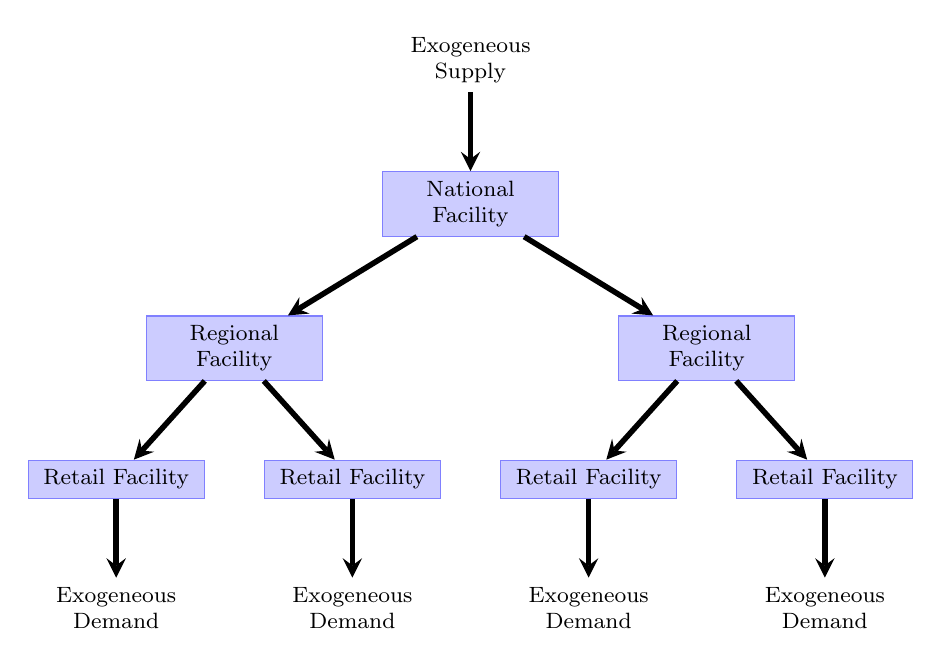
\begin{tikzpicture}
    [exoge/.style={rectangle,minimum width=20mm,align=center,
                   text width=20mm,font=\footnotesize},
     node distance=10mm]
  % facilities
  \node[exoge] (sup)                               {Exogeneous Supply};
  \node[facility] (nat)  [below=of sup]               {National Facility};
  \node[facility] (reg1) [below=of nat,xshift=-30mm]  {Regional Facility};
  \node[facility] (reg2) [below=of nat,xshift=30mm]   {Regional Facility};
  \node[facility] (ret1) [below=of reg1,xshift=-15mm] {Retail Facility};
  \node[facility] (ret2) [below=of reg1,xshift=15mm]  {Retail Facility};
  \node[facility] (ret3) [below=of reg2,xshift=-15mm] {Retail Facility};
  \node[facility] (ret4) [below=of reg2,xshift=15mm]  {Retail Facility};
  \node[exoge] (dem1) [below=of ret1]              {Exogeneous Demand};
  \node[exoge] (dem2) [below=of ret2]              {Exogeneous Demand};
  \node[exoge] (dem3) [below=of ret3]              {Exogeneous Demand};
  \node[exoge] (dem4) [below=of ret4]              {Exogeneous Demand};

  % inventory flows
  \draw[medarrow] (sup) -- (nat);
  \draw[medarrow] (nat) -- (reg1);
  \draw[medarrow] (nat) -- (reg2);
  \draw[medarrow] (reg1) -- (ret1);
  \draw[medarrow] (reg1) -- (ret2);
  \draw[medarrow] (reg2) -- (ret3);
  \draw[medarrow] (reg2) -- (ret4);
  \draw[medarrow] (ret1) -- (dem1);
  \draw[medarrow] (ret2) -- (dem2);
  \draw[medarrow] (ret3) -- (dem3);
  \draw[medarrow] (ret4) -- (dem4);
\end{tikzpicture}
\caption{Example to illustrate the supply chain topology of \scs.
Arrows denote the direction of inventory flows.}
\label{figure:conceptual-model->supply-chain-topology}
\end{figure}




\section{Exogenous Supply and Demand}
\label{section:conceptual-model->supply-and-demand}

The exogenous supply arrives at the \entity{national facility},
while the exogenous demand arrives at each \entity{retail facility}.
This is illustrated in
\autoref{figure:conceptual-model->supply-chain-topology}.

The \entity{national supply schedule}
specifies both the timing and the quantity
of inventory arriving at the \entity{national facility}.
It is assumed that the supply of inventory
received by the \entity{national facility} is exogenous.

At each \entity{retail facility},
inventory is depleted by the demand
induced by customers who arrive at the facility.
In general, the demand is random,
and generated from a probability distribution
which is specified by the \entity{demand model}.
The demand is assumed to be exogenous,
i.e.\ it is statistically independent
of the state of the supply chain
and of the inventory replenishment policy used.

In the supply chain management literature,
there are two different types of assumptions made about unmet demand:
either unmet demand is backordered
(i.e.\ customers remain waiting for the product
and the demand is satisfied when inventory arrives in a future period),
or unment demand is lost forever.
\scs\ assumes that unmet demand is lost forever.

To define the \entity{demand model} more precisely,
let us denote by $\rvd_{rt}$
the random quantity demanded at retail facility $r$ during period $t$.
The \entity{demand model} specifies the joint probability distribution
of the demand for each retail facility and each period,
i.e.\ the set of random variables $\{\rvd_{rt}\}_{r,t}$
over all retail facilities $r$ and all periods $t$.

The \entity{demand model} is also able to provide
a demand forecast of future demand $\rvd_{ru}$
given all information revealed by the current time period $t$,
which we denote by $\info_t$.
Certain \entity{inventory replenishment policies}
may use compute a replenishment quantity
that depends on the demand forecasts $\rvd_{ru}$.
For example,
an order-up-to policy
that orders up to the mean demand in the next 12 periods
would ship a replenishment quantity given by
\begin{align*}
    q
  &=
    \text{expected demand in } [t, t+12) - \text{inventory position}_t
\\
  &=
    \sum_{u=t}^{t+11} \cEX{\rvd_{ru}}{\info_t} - ip_t.
\end{align*}






\section{Inventory Replenishment Process}
\label{section:conceptual-model->inventory-replenishment} 

We define the basic inventory replenishment process
in \autoref{conceptual-model->inventory-replenishment:generic-(supplier-customer)}.
We introduce inventory replenishment constraints
in \autoref{section:conceptual-model->inventory-replenishment-constraints}.
The \scs\ supply chain can be operated
in either an intermediate stocking configuration
or a cross-docking configuration.
We define the inventory replenishment process
for an intermediate stocking configuration
in \autoref{subsection:conceptual-model->inventory-replenishment->istock},
while we define the process
for a cross-docking configuration
in \autoref{subsection:conceptual-model->inventory-replenishment->xdock}.






\subsection{Basic Inventory Replenishment Process}
\label{conceptual-model->inventory-replenishment:generic-(supplier-customer)}

In this section,
we define the basic inventory replenishment process,
i.e.\ the process by which a customer facility
receives inventory replenishment from a dedicated supplier facility.
We refer to this arrangement as a (supplier, customer) relationship.

In order to define the inventory replenishment process,
we first need to define the following entities:
\begin{description}
  \item[Report]
      The \entity{report} submitted by the customer facility
      is a record of information that is relevant
      in calculating a replenishment shipment quantity, including:
      \begin{itemize}
        \item The customer facility's current inventory level
        \item Shipments in the inventory pipeline to the customer facility
        \item Past demand and consumption at the customer facility
      \end{itemize}
  \item[Replenishment policy]
      When a supplier facility has received a \entity{report}
      from a customer facility,
      the supplier facility uses the \entity{replenishment policy}
      to calculate the shipment quantity
      based on a subset of the following inputs:
      \begin{itemize}
        \item the received \entity{report}
        \item the forecast for future \entity{demand} at the customer
        \item the \entity{lead time} forecast for past, current and future
            shipments to the customer
      \end{itemize}
      A \entity{replenishment policy} need not take into account
      all of the above factors to compute a shipment quantity.
      For example, an order-up-to policy
      only depends on the customer facility \entity{report}.
  \item[Shipment]
      A shipment is some number of units of the product
      that is packaged by the supplier facility into a common lot
      and shipped to the customer facility.
\end{description}

The basic inventory replenishment process is the following:
\begin{enumerate}
  \item The customer facility sends a \entity{report}
      to its supplier facility.
  \item The supplier facility processes the \entity{report}
      according to the \entity{inventory replenishment policy}
      and computes a replenishment quantity,
      and makes an \entity{shipment} to the customer facility.
  \item The \entity{shipment} arrives at the customer facility.
\end{enumerate}
This is illustrated in
\autoref{figure:inventory-replenishment-process}.


\begin{figure}[h!]
\centering
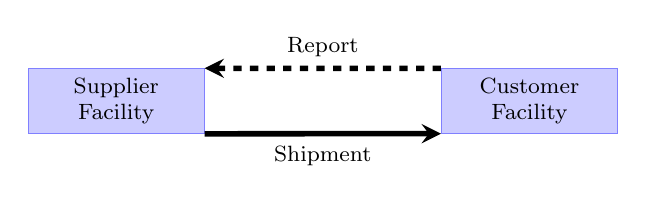
\begin{tikzpicture}[node distance=30mm]
  \node[facility] (sup)                 {Supplier Facility};
  \node[facility] (cust) [right=of sup] {Customer Facility};

  \draw[medarrow,dashed]
      (cust.north west) -- 
      node[auto,mail,above] {Report}
      (sup.north east);

  \draw[medarrow]
      (sup.south east) -- 
      node[auto,mail,below] {Shipment}
      (cust.south west);
\end{tikzpicture}
\\[5mm]
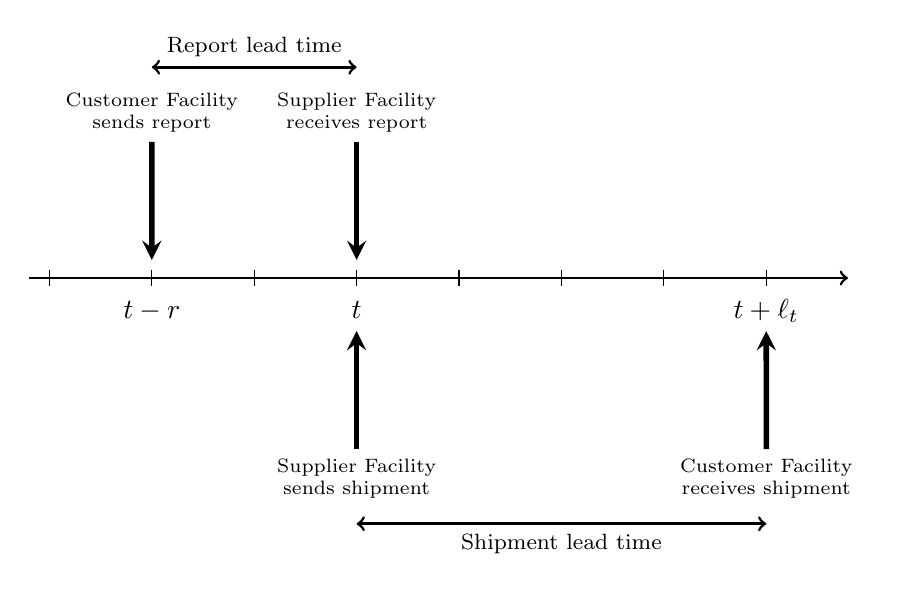
\begin{tikzpicture}[
    xscale=1.3,
    node distance=15mm,
    ]
  % space between event labels and interval arrow
  \def \myyshift{2mm}

  \foreach \i in {-3,...,4} {
    \draw (\i cm,3pt)
        node (uptic\i) {}
        -- (\i cm,-3pt)
        node (downtic\i) {};
  }
  \draw[->,line width=1pt] (-3.2,0) -- (4.8,0);

  \node[timelabel]
       (reportSentTime) at (downtic-2) {$t - r$};
  \node[event]    (reportSentLabel) [above=of uptic-2]
      {Customer Facility sends report};
  \draw[medarrow] (reportSentLabel) -- (uptic-2);

  \node[timelabel]
      (reportSentTime) at (downtic0) {$t$};
  \node[event]     (reportReceivedLabel) [above=of uptic0]
      {Supplier Facility receives report};
  \draw[medarrow] (reportReceivedLabel) -- (uptic0);
  \node[event] (shipmentSentLabel) [below=of reportSentTime]
      {Supplier Facility sends shipment};
  \draw[medarrow] (shipmentSentLabel) -- (reportSentTime);

  \node[timelabel]
      (shipmentSentTime) at (downtic4) {$t + \ell_t$};
  \node[event] (shipmentReceivedLabel) [below=of shipmentSentTime]
      {Customer Facility receives shipment};
  \draw[medarrow] (shipmentReceivedLabel) -- (shipmentSentTime);

  \draw[interval]
      ([yshift=\myyshift]reportSentLabel.north) --
      node[auto,above] {Report lead time}
      ([yshift=\myyshift]reportReceivedLabel.north);

  \draw[interval]
      ([yshift=-\myyshift]shipmentSentLabel.south) --
      node[auto,below] {Shipment lead time}
      ([yshift=-\myyshift]shipmentReceivedLabel.south);
\end{tikzpicture}
\caption{Illustration of the inventory replenishment process.}
\label{figure:inventory-replenishment-process}
\end{figure}

In order to define the schedule of events
in the inventory replenishment process,
we first need to define the following concepts:
\begin{description}
  \item[Shipment schedule] 
      The \entity{shipment schedule} indicates which are the periods
      in which the supplier facility can make a \entity{shipment}
      to the customer facility.
  \item[Shipment lead time]
      The \entity{shipment} lead time is the number of periods of delay
      between the supplier facility sending a \entity{shipment}
      and the customer facility receiving the \entity{shipment}.
      The \entity{shipment} lead time may be random
      and depend on the period in which the \entity{shipment} is sent.
      We denote the \entity{shipment} lead time at period $t$
      by $\ell_t$ periods.
  \item[Report lead time]
      The \entity{report} lead time is the number of periods of delay
      between the customer facility sending a \entity{report}
      and the customer facility receiving the \entity{report}.
      The \entity{report} lead time is assumed to be constant,
      and we denote the \entity{report} lead time by $r$ periods.
\end{description}

Suppose that the \entity{shipment schedule}
indicates that the supplier facility
is eligible to make a \entity{shipment}
to the customer facility at the beginning of period $t$.
The schedule of events in the inventory replenishment process
is defined as follows:
\begin{description}
  \item[Period $t - r$:]
      The customer facility submits a \entity{report}
      to the supplier facility.
  \item[Period $t$:]
      The supplier facility receives the \entity{report}
      from the customer facility,
      and makes a \entity{shipment} to the customer facility.
  \item[Period $t + \ell_t$:]
      The customer facility receives the \entity{shipment}
      from the supplier facility.
\end{description}
This is illustrated in 
\autoref{figure:inventory-replenishment-process}.






\subsection{Inventory Replenishment Constraints}
\label{section:conceptual-model->inventory-replenishment-constraints}

For the sake of clarity,
we will refer to shipments
from the \entity{national facility} to \entity{regional facilities}
as \emph{primary distribution};
and refer to shipments
from \entity{regional facilities} to \entity{retail facilities}
as \emph{secondary distribution}.
This is illustrated in
\autoref{figure:conceptual-model->inventory-replenishment-constraints->primary-secondary-distribution}.

\begin{figure}[h!]
  \centering
  \def \myyshift {0mm}
  \tikzset{node distance=25mm}
  \centering
  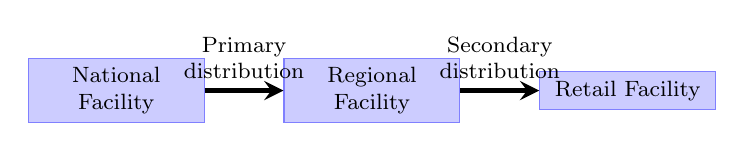
\begin{tikzpicture}
    % Facilities
    \node[facility] (nat)                {National Facility};
    \node[facility] (reg) [right=of nat] {Regional Facility};
    \node[facility] (ret) [right=of reg] {Retail Facility};

    % Inventory flows
    \draw[invflow]
        (nat) -- 
        node[auto,above,text width=20mm,align=center,font=\footnotesize]
            {Primary distribution}
        (reg);
    \draw[invflow]
        (reg) -- 
        node[auto,above,text width=20mm,align=center,font=\footnotesize]
            {Secondary distribution}
        (ret);
  \end{tikzpicture}
  \caption{Illustration of primary and secondary distribution.
    Arrows denote the direction of inventory flows.
  }
  \label{figure:conceptual-model->inventory-replenishment-constraints->primary-secondary-distribution}
\end{figure}



In the same way,
we can define the primary and secondary \entity{report} lead times,
and the primary and secondary \entity{shipment} lead times,
and primary and secondary \entity{shipment schedules}.
This is illustrated in
\autoref{figure:conceptual-model->inventory-replenishment:primary-secondary-lead-times}.

\begin{figure}[h!]
  \centering
  \def \myyshift {0mm}
  \tikzset{node distance=25mm}
  \centering
  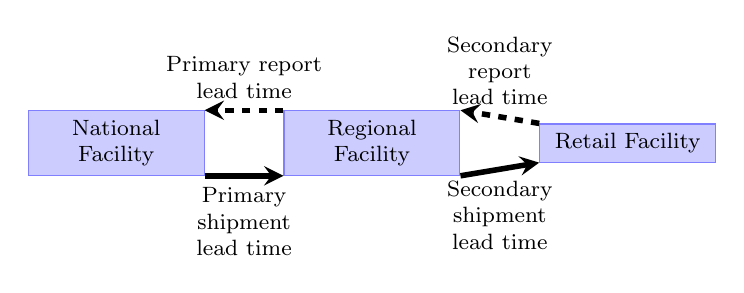
\begin{tikzpicture}
    % Facilities
    \node[facility] (nat)                {National Facility};
    \node[facility] (reg) [right=of nat] {Regional Facility};
    \node[facility] (ret) [right=of reg] {Retail Facility};

    % Report flows
    \draw[reportflow]
        (reg.north west) -- 
        node[auto,above,text width=20mm,align=center,font=\footnotesize]
            {Primary report lead time}
        (nat.north east);

    \draw[reportflow]
        (ret.north west) -- 
        node[auto,above,text width=20mm,align=center,font=\footnotesize]
            {Secondary report lead time}
        (reg.north east);
    % Inventory flows
    \draw[invflow]
        (nat.south east) -- 
        node[auto,below,text width=20mm,align=center,font=\footnotesize]
            {Primary shipment lead time}
        (reg.south west);
    \draw[invflow]
        (reg.south east) -- 
        node[auto,below,text width=20mm,align=center,font=\footnotesize]
            {Secondary shipment lead time}
        (ret.south west);
  \end{tikzpicture}
  \caption{Illustration of primary/secondary report/shipment lead times.}
  \label{figure:conceptual-model->inventory-replenishment:primary-secondary-lead-times}
\end{figure}




It is assumed that the primary and secondary \entity{shipment schedules}
are invariable.

It is assumed that the \entity{report} lead time is constant and deterministic,
and that the primary \entity{report} lead time
is equal to the secondary \entity{report} lead time.

In general, the \entity{shipment} lead times are random
and can be non-stationary.





\subsection{Intermediate Stocking Configuration}
\label{subsection:conceptual-model->inventory-replenishment->istock}

In an \entity{intermediate stocking configuration},
each \entity{regional facility} maintains a common pool of inventory,
from which replenishment shipments are made
to all \entity{retail facilities} in its region.
This is illustrated in
\autoref{figure:conceptual-model->istock-vs-xdock}.

\begin{figure}[h!]
\centering
\def \myyshift {3mm}
\tikzset{node distance=25mm}
\begin{subfigure}{\textwidth}
  \centering
  \begin{tikzpicture}
    % Facilities
    \node[facility] (nat)                {National Facility};
    \node[facility] (reg) [right=of nat] {Regional Facility};
    \node[facility] (ret) [right=of reg] {Retail Facility};

    % Reports
    \draw[->,line width=2pt,dashed]
        ([yshift=\myyshift]ret.west) --
        node[auto,mail,above] {Report}
        ([yshift=\myyshift]reg.east);
    \draw[->,line width=2pt,dashed]
        ([yshift=\myyshift]reg.west) --
        node[auto,mail,above] {Report}
        ([yshift=\myyshift]nat.east);

    % Shipments
    \draw[->,line width=2pt]
        ([yshift=-\myyshift]nat.east) --
        node[auto,mail,below] {Shipment}
        ([yshift=-\myyshift]reg.west);
    \draw[->,line width=2pt]
        ([yshift=-\myyshift]reg.east) --
        node[auto,mail,below] {Shipment}
        ([yshift=-\myyshift]ret.west);
  \end{tikzpicture}
  \captionof{figure}{Intermediate stocking configuration}
\end{subfigure}
\\
\begin{subfigure}{\textwidth}
  \centering
  \begin{tikzpicture}
    \node[facility] (nat)                {National Facility};
    \node[facility,fill opacity=0.2] (reg) [right=of nat] {Regional Facility};
    \node[facility] (ret) [right=of reg] {Retail Facility};

    % Report
    \draw[->,line width=2pt,dashed]
        ([yshift=\myyshift]ret.west) --
        node[auto,mail,above] {Report}
        ([yshift=\myyshift]nat.east);

    % Shipment
    \draw[->,line width=2pt]
        ([yshift=-\myyshift]nat.east) --
        node[auto,mail,below] {Shipment}
        ([yshift=-\myyshift]ret.west);
  \end{tikzpicture}
  \captionof{figure}{Cross-docking configuration}
\end{subfigure}
\caption{
  Illustration of the flow of information and inventory
  in the intermediate stocking and cross-docking
  supply chain configurations.
}
\label{figure:conceptual-model->istock-vs-xdock}
\end{figure}



In an intermediate stocking configuration,
there are two types of (supplier, customer) relationships.
\begin{itemize}
\item
In the (\entity{national facility}, \entity{regional facility}) relationship,
the \entity{report} lead time is the primary \entity{report} lead time,
the \entity{shipment} lead time is the primary \entity{report} lead time,
and the \entity{shipment schedule} is the primary \entity{shipment schedule}.
\item
In the (\entity{regional facility}, \entity{retail facility}) relationship,
the \entity{report} lead time is the secondary \entity{report} lead time,
the \entity{shipment} lead time is the secondary \entity{report} lead time,
and the \entity{shipment schedule} is the secondary \entity{shipment schedule}.
\end{itemize}





\subsection{Cross-docking Replenishment}
\label{subsection:conceptual-model->inventory-replenishment->xdock}

In a cross-docking configuration,
a \entity{retail facility} submits a \entity{report}
which passes through its respective \entity{regional facility}
to the \entity{national facility};
upon receipt of the \entity{report},
the \entity{national facility} makes a \entity{shipment}
that passes through the \entity{regional facility}
to be received by the \entity{retail facility}.
When the supply chain is operated in a cross-docking configuration,
Any inventory held in a \entity{regional facility} is consigned
for a particular \entity{retail facility}.
This is illustrated in
\autoref{figure:conceptual-model->istock-vs-xdock}.

In a cross-docking configuration,
there is only onetype of (supplier, customer) relationship
which is (\entity{national facility}, \entity{retail facility}).
It is assumed that once a \entity{regional facility}
receives a \entity{shipment} intended for
a \entity{retail facility} in its region,
the \entity{regional facility} immediately initiates delivery,
so the \entity{shipment} is received at the \entity{retail facility}
after the secondary \entity{shipment} lead time.
In this relationship,
the \entity{report} lead time is
the sum of the primary and secondary \entity{report} lead times;
the \entity{shipment} lead time is
the sum of the primary and secondary \entity{shipment} lead times;
and the \entity{shipment schedule} is
the primary \entity{shipment schedule}.





\section{Sequence of Events in Each Period}
\label{section:conceptual-model->sequence-of-events}

The supply chain is operated
in either an \entity{intermediate stocking} configuration
or a \entity{cross-docking configuration}.
In either configuration,
the sequence of events in each period follows the following pattern:
\begin{enumerate}
\item
\textbf{Customer facilities submit reports.}
For each (supplier, customer) relationship,
if the current period is a reporting period,
then a customer facility submits a \entity{report} to a supplier facility.
The order of \entity{report} submission
is from facilities in the lowest tier to the highest tier,
i.e.\ \entity{retail facilities} submit \entity{reports}
before \entity{regional facilities}.
\item
\textbf{Facilities receive shipments and make shipments.}
For each facility,
receive \entity{shipments} and make \entity{shipments} (if applicable).
First, the exogeneous supplier makes a \entity{shipment}
to the \entity{national facility}
according to the \entity{national replenishment policy}.
Then in the order of highest tier to the lowest tier,
facilities receive \entity{shipments}
and make \entity{shipments} (if applicable).
In other words,
first the \entity{national facility} receives and makes \entity{shipments},
then the \entity{regional facilities} receive and make \entity{shipments},
and finally the \entity{retail facilities} receive \entity{shipments}.
\item
\textbf{Customers arrive at retail facilities.}
Customers arrive at \entity{retail facilities},
depleting inventory and incurring unmet demand (if applicable).
\end{enumerate}



The pseudocode for the detailed sequence of events
in an \entity{intermediate stocking} configuration
is shown in \autoref{algo:conceptual-model->sequence->istock};
while the pseudocode for the detailed sequence of events
in an \entity{cross-docking} configuration
is shown in \autoref{algo:conceptual-model->sequence->xdock}.


\begin{algorithm}[h!]
\begin{algorithmic}
\State $t \gets$ start period
\While{$t \leq$ end period}
    \State \algocomment{submit reports}
    \ForAll{(regional, retail) is a SCR}
        \If{is reporting period for customer facility}
            \State customer facility submits report to supplier facility
        \EndIf
    \EndFor
    \ForAll{(national, regional) is a SCR}
        \If{is reporting period for customer facility}
            \State customer facility submits report to supplier facility
        \EndIf
    \EndFor
    \State \algocomment{receive shipments and make shipments}
    \State exogeneous supplier
        makes {shipments} to {national facility}
    \State {national facility} receives {shipments}
    \ForAll{regional facility}
        \State {regional facility} receives {shipments}
        \State {regional facility} makes {shipments}
            to {retail facilities}
    \EndFor
    \ForAll{retail facility}
        \State {retail facility} receives {shipments}
    \EndFor
    \State \algocomment{demand arrives}
    \ForAll{retail facility}
        \State demand arrives at {retail facility}
    \EndFor
\EndWhile
\end{algorithmic}
\caption{Pseudocode for sequence of events in each period
for the intermediate stocking simulator.}
\label{algo:conceptual-model->sequence->istock}
\end{algorithm}





\begin{algorithm}[h!]
\begin{algorithmic}
\State $t \gets$ start period
\While{$t \leq$ end period}
    \State \algocomment{submit reports}
    \ForAll{retail facility}
        \If{is reporting period for customer facility}
            \State retail facility submits report to national facility
        \EndIf
    \EndFor
    \State \algocomment{receive shipments and make shipments}
    \State exogeneous supplier
        makes {shipments} to {national facility}
    \State {national facility} receives {shipments}
    \State {national facility} makes {shipments}
            to {retail facilities}
    \ForAll{retail facility}
        \State {retail facility} receives {shipments}
    \EndFor
    \State \algocomment{demand arrives}
    \ForAll{retail facility}
        \State demand arrives at {retail facility}
    \EndFor
\EndWhile
\end{algorithmic}
\caption{Pseudocode for sequence of events in each period
for the cross-docking simulator.}
\label{algo:conceptual-model->sequence->xdock}
\end{algorithm}

\clearpage





\section{Simulation Replication}
\label{section:conceptual-model->simulator-replication}

A simulation run of \scs\ can be characterized by three separate components:
\begin{itemize}
  \item Exogeneous components
  \item Replenishment process components
  \item Initial state
  \item Simulation run parameters
\end{itemize}

The following components of the supply chain
are assumed to be exogeneous,
and independent of the replenishment process
and the simulation run parameters:
\begin{itemize}
  \item supply chain topology
  \item shipment lead time model
  \item report lead time model
  \item demand model model
  \item replenishment policy for national facility
  \item national facility to regional facility shipment schedule
\end{itemize}

The replenishment process depends on the supply chain configuration.
\begin{itemize}
  \item
    In an intermediate stocking configuration,
    the replenishment process is defined by:
    \begin{itemize}
      \item replenishment policy for regional facilities
      \item replenishment policy for retail facilities
      \item regional facility to retail facility shipment schedule
    \end{itemize}
  \item
    In a cross-docking configuration,
    the replenishment process depends only on the retail replenishment policy.
\end{itemize}

The initial state of the supply chain is defined by
\begin{itemize}
  \item The inventory level at the \entity{national facility}
  \item The inventory level at each \entity{regional facility}
    (only in the intermediate stocking configuration)
  \item The inventory level at each \entity{retail facility}
\end{itemize}

The simulation run parameters are:
\begin{itemize}
  \item initial inventory level at national, regional, retail facilities
  \item simulation start and end periods
  \item random seed (i.e.\ the number used to initialize
    a pseudorandom number generator)
\end{itemize}





\chapter[Computer Model (\scs)]{Computer Model of Supply Chain}
\label{chapter:implementation}

\section{Overview}

In this chapter,
we describe the computer model of the supply chain.
In other words,
we describe the software implementation
of the conceptual model of the supply chain
which was described in \autoref{chapter:conceptual-model}.


In \autoref{section:scs->computer-model->java-programming},
we give the reader a brief introduction
to the Java\texttrademark\  programming language.
In \autoref{section:scs->computer-model->software-engineering-tools}
we explain some of the software engineering tools
that we used in the software implementation and documentation of \scs.
In \autoref{section:scs->computer-model->controller-objects},
we describe the controller objects which implement the supply chain logic
which was described in \autoref{chapter:conceptual-model}.
The following three sections each describe
the computer implementation of an element in the supply chain,
the supply chain topology in
\autoref{section:scs->computer-model->supply-chain-topology},
the exogeneous supply and demand in 
\autoref{section:scs->computer-model->supply-and-demand},
the inventory replenishment process in
\autoref{section:scs->computer-model->replenishment-process}.
While reading these three sections,
it may be useful for the reader to refer to the
corresponding section in \autoref{chapter:conceptual-model}.
Finally, in \autoref{section:scs->computer-model->design-of-experiments}
we describe how to design computer experiments.

\paragraph{Notation}
In this chapter,
we use typewriter font, e.g.\ \code{NationalFacility},
to denote the name of a Java class.
The code lisitings, e.g.\ \autoref{figure:hello-world}
also use the typewriter font.





\section{Essentials of Java Programming}
\label{section:scs->computer-model->java-programming}

\subsection{Hello World}

In the Java programming language,
every application must contain a \code{main} method.
This is the entry point of the application
and will subsequently invoke all the other methods required by your program.
For example, the famous ``Hello World'' program in Java
is shown in \autoref{figure:hello-world}.
For more information about the \code{main} method,
see \citet{java-tutorials->hello-world}.



\begin{figure}[h!]
\begin{lstlisting}
public class HelloWorld {
    public static void main(String[] args) {
        System.out.println("Hello world");
    }
}
\end{lstlisting}
\caption{The famous ``Hello world'' program in Java}
\label{figure:hello-world}
\end{figure}





\subsection{Object-Oriented Programming}

In an object-oriented programming paradigm,
the computer program creates software objects,
which are models of real-world objects.
A software object has an internal state
and methods which model
the interaction of the real-world object
with other objects or the external environment.
The computer program accomplishes its goal
by guiding the interaction of its software objects.

In the Java programming language,
a software object is created by instantiating a class.
A \emph{class} is a blueprint or prototype that defines
how to create a software object,
and what is the state and behavior of the software object.
For example, the code in
\autoref{figure:scs->computer-model->dog-class}
is an example of a class definition for the class \code{Dog}.
The class definition
defines the state of a software dog object (the dog's breed and name)
and its behavior (the dog can print its breed and name to the console).

\begin{figure}[h!]
\begin{lstlisting}
public class Dog {
    private String breed;
    private String name;

    public Dog(String breed, String name) {
        this.breed = breed;
        this.name = name;
    }

    public void print() {
        System.out.printf("Dog{breed=%s,name=%s}%n", breed, name);
    }
}
\end{lstlisting}
\caption{Definition of the class \protect\code{Dog}.}
\label{figure:scs->computer-model->dog-class}
\end{figure}

For more information about OOP concepts,
we refer the reader to \citet{java-tutorials->oop-concepts}.


\scs\ is written using an OOP paradigm.
In other words, each entity in the conceptual model of the supply chain
is modeled by a software object in the simulation
(see \autoref{table:scs->computer-model->supply-chain-topology}).

\begin{table}[h!]
\centering
\small
\begin{tabular}{ll}
\toprule
  Java class & Conceptual entity \\
\midrule
    \code{Topology}
  &
    Supply chain topology
\\
    \code{NationalFacility}
  &
    National facility
\\
    \code{RegionalFacility}
  &
    Regional facility
\\
    \code{RetailFacility}
  &
    Retail facility
\\
    \code{Shipment}
  &
    Shipment
\\
    \code{Report}
  &
    Report
\\
    \code{NationalSupplySchedule}
  &
    Supply schedule for national facility
\\
    \code{DemandModel}
  &
    Demand model
\\
    \code{LeadTime}
  &
    Lead time model
\\
    \code{AbstractReplenishmentPolicy}
  &
    Inventory replenishment policy
\\
\bottomrule
\end{tabular}
\caption{Java classes that implement conceptual entities
in the supply chain topology.}
\label{table:scs->computer-model->supply-chain-topology}
\end{table}




Java supports an object-oriented programming concept
which is refered to as \emph{inheritance}.
This is explained by the Oracle lesson on inheritance
\cite{java-tutorials->inheritance}
as follows:
\begin{quotation}
Certain objects can have common states and behaviors.
For example, mountain bikes, road bikes, and tandem bikes
share certain characteristics of bicycles such as
current speed and current gear.
Yet each also defines additional features that make them different.
Object-oriented programming allows classes to \emph{inherit}
commonly used state and behavior from other classes.
In this example,
\code{Bicycle} now becomes the superclass
of \code{MountainBike}, \code{RoadBike}, and \code{TandemBike}.
\end{quotation}




\subsection{Packages}


A large software project can have a large number of Java classes.
For example, the implementation of \scs\ has more than 80 classes.
If the classes were not organized in some way,
it would be hard to for a programmer
to know what classes are related
and how classes work together to achieve a desired functionality.

In order to manage large and complex software projects,
people use a software design technique known as \emph{modular programming}.
With modular programming, the software project
is divided into distinct modules,
such that each module is responsible for
one and only one aspect of the desired functionality.

Java supports modular programming through its package mechanism
\citep{java-tutorials->packages}.
The computer implementation of \scs\ is composed of the packages
shown in \autoref{table:scs->computer-model->packages}.

\begin{table}[h!]
\centering
\small
\begin{tabular}{ll}
\toprule
  Java package & Concern \\
\midrule
    \code{com.gly.random}
  & Random variables
\\
    \code{com.gly.util}
  & Utility classes
\\
    \code{com.gly.scs.data}
  & The repository classes
\\
    \code{com.gly.scs.demand}
  & Demand models
\\
    \code{com.gly.scs.domain}
  & Entities in the supply chain
\\
    \code{com.gly.scs.leadtime}
  & Lead time models
\\
    \code{com.gly.scs.main}
  & Classes with \code{main} methods
\\
    \code{com.gly.replen}
  & Replenishment policies
\\
    \code{com.gly.scs.sched}
  & Shipment schedules
\\
    \code{com.gly.sim}
  & Controller objects
\\
\bottomrule
\end{tabular}
\caption{Packages in the \scs\ computer code.}
\label{table:scs->computer-model->packages}
\end{table}





\section{Software Engineering Tools}
\label{section:scs->computer-model->software-engineering-tools}

\subsection{Unified Modeling Language}

In this chapter,
we use UML class diagrams to visualize the fields and methods of classes
and the interrelationships between classes.
UML class diagrams are a standard tool in the field of software engineering.
Wikipedia \citep{wikipedia->uml}
describes the Unified Modeling Language (UML) as follows:
\begin{quote}
The Unified Modeling Language (UML) is a general-purpose modeling language in the field of software engineering, which is designed to provide a standard way to visualize the design of a system.
\end{quote}

In particular, one of the components of UML is the UML class diagram
which Wikipedia \citep{wikipedia->uml-class-diagram} desribes as follows:
\begin{quote}
In software engineering, a class diagram in the Unified Modeling Language (UML) is a type of static structure diagram that describes the structure of a system by showing the system's classes, their attributes, operations (or methods), and the relationships among objects.
\end{quote}

A simple example of the UML class diagram of the \code{Dog} class
defined above in 
\autoref{figure:scs->computer-model->dog-class}
is shown in
\autoref{figure:scs-computer-model->dog-uml-class-diagram}.

It can be seen that a class is represented by a rectangle
which is divided into three parts:
\begin{itemize}
\item
The top part contains the name of the class.
\item
The middle part contains the attributes of the class.
\item
The bottom part gives the methods or operations the class can take or undertake.
\end{itemize}

\begin{figure}[h!]
\centering
\begin{myuml}
  \begin{class}[text width=8cm]{Dog}{0,0}
    \attribute{-breed : String}
    \attribute{-name : String}
    \operation{+print() : void}
  \end{class}
\end{myuml}
\caption{UML class diagram of the \protect\code{Dog} class.}
\label{figure:scs-computer-model->dog-uml-class-diagram}
\end{figure}






\subsection{Software Design Patterns}

In the implementation of \scs,
we make use of \emph{software design patterns}.
Wikipedia explains what are software design patterns
and why they are used:
\begin{quotation}
In software engineering,
a design pattern is a general reusable solution
to a commonly occurring problem within a given context in software design.
A design pattern is a description or template
for how to solve a problem that can be used in many different situations.
Patterns are formalized best practices
that the programmer can use to solve common problems
when designing an application or system.
\end{quotation}

For more information about software design patterns,
refer to the seminal book on design patterns: \cite{gang-of-four-1994}.





\subsubsection{Builder design pattern}

The \emph{builder design pattern}
is useful when the construction of an object requires many parameters.
The builder design pattern uses a builder object
which receives each initialization parameter step by step
and then returns the resulting constructed object at once.

We illustrate the use of the builder design pattern using a simple example
of a \code{Person} class,
which has fields \code{firstName}, \code{lastName} and \code{salutation}.

\begin{lstlisting}
public class Person {
    private String firstName;
    private String lastName;
    private String salutation;
}
\end{lstlisting}

The traditional Java constructor approach might define a constructor
\begin{lstlisting}
Person(String firstName, String lastName, String salutation)
\end{lstlisting}
However, if a user is not careful,
the user may call the constructor with the wrong order of parameters:
\begin{lstlisting}
Person person = new Person("Barack", "Obama", "President") // right!
Person person = new Person("President", "Barack", "Obama") // wrong!
\end{lstlisting}

In contrast, a builder object can be used
to instantiate a \code{Person} object as follows:
\begin{lstlisting}
Person person = new Person.Builder()
        .withFirstName("Barack")
        .withLastName("Obama")
        .withSalutation("President")
        .build();
\end{lstlisting}

As the previous code snippets show,
using the builder design pattern makes the code more readable
and less error-prone.

\scs\ uses the builder design pattern to create objects
which require many parameters in their creation,
e.g.\ the classes \code{Shipment}, \code{IstockSimulator}, among others.
For instance, the code to create a \code{Shipment} object
is shown in \autoref{figure:scs->computer-model->create-a-Shipment-object}.

\begin{figure}[h!]
\begin{lstlisting}
// create a new shipment object
Shipment shipment = new Shipment.Builder()
.withPeriodReceived(period + thisLeadTime.getLeadTime(to.getId(), period))
.withPeriodSent(period)
.withQuantity(quantity)
.withTo(to)
.build();
\end{lstlisting}
\caption{Code to create a \code{Shipment} object,
which uses the builder design pattern.}
\label{figure:scs->computer-model->create-a-Shipment-object}
\end{figure}
created using.





\subsubsection{Abstract factory design pattern}

The \emph{abstract factory design pattern} is a creational design pattern.
As defined by \cite{gang-of-four-1994},
the goal of using the abstract factory design pattern is to
``provides an interface for creating families
of related or dependent objects without specifying their concrete classes.''

We illustrate the abstract factory design pattern using the following example.

Suppose that we were writing
a graphical design application for drawing shapes.
The abstract \code{Shape} class
defines the \code{draw} and \code{move} methods
which must be implemented by its concrete subclasses:
\code{Circle}, \code{Triangle} and \code{Rectangle}.
We can define an abstract \code{ShapeFactory} class
with an abstract method \code{createShape}.
Then we can define subclasses of the \code{ShapeFactory} class
as factories for each of the shapes:
\code{CircleFactory}, \code{TriangleFactory}, \code{RectangleFactory}.
By using the abstract factory design pattern,
we can use the same code
in the source code of the graphical design application
for drawing shapes.
When the user specifies which shape to draw,
the user interface object can create
a corresponding \code{ShapeFactory} object
which is passed to the graphical design object.
The code in the controller object might look like the following:
\begin{lstlisting}
ShapeFactory shapeFactory = 
        userInterface.getShapeFactoryFromUser();
graphicalDesign.drawShape(shapeFactory.createShape());
\end{lstlisting}

\scs\ uses the abstract factory design pattern
in the controller objects
(see \autoref{section:scs->computer-model->controller-objects})
to create the demand model object and lead time model objects.





\subsubsection{Repository Design Pattern}

Using the terminology of \cite{evans-2004},
the \emph{repository design pattern}
is used to create an abstraction between the domain and data layer.
We do not define what is a domain layer or a data layer.
(We refer interested readers to the book.)
Instead, to illustrate how the repository design pattern works,
we consider the example of a shipment repository.
The \code{ShipmentRepository} class defines an object
which acts as a repository for all \code{Shipment} objects,
i.e.\ all \code{Shipment} objects
are stored within the \code{ShipmentRepository} class.
The \code{ShipmentRepository} class has methods
both for adding new \code{Shipment} objects into the repository,
and for removing all \code{Shipment} objects matching certain criteria.
Therefore, the \code{ShipmentRepository} class
hides the internal details of how it manages \code{Shipment} objects,
and allows other classes to use
the interface defined by the \code{ShipmentRepository} class
to add, access or remove \code{Shipment} objects.
This is advantageous because it encapsulates all the code
related to the storage and retrieval of \code{Shipment} objects
in a single \code{ShipmentRepository} class,
which we can be test systematically.

\scs\ uses repository objects to manage
facilities (\code{FacilityRepository}),
shipments (\code{ShipmentRepository})
and reports (\code{ReportRepository}).




\section{Controller Objects}
\label{section:scs->computer-model->controller-objects}

In an OOP paradigm,
every domain object (entity in the conceptual model of the supply chain)
is represented by a software object in the computer code.
Therefore, we define software objects such as
\code{RetailFacility}, \code{Shipment} and \code{Report}
to model entities in the domain which is a supply chain.
We use \emph{controller objects}
in order to coordinate the interaction
of the domain objects in the supply chain
and to implement the control logic specified in the Conceptual Model chapter.
For example, the controller object
gets a \code{Report} object from the customer facility object,
and arranges for the \code{Report} object
to be received by the supplier facility
after the \code{Report} lead time specified by the
\code{ReplenishmentPolicy} object.

\begin{figure}[h!]
\centering
\begin{myuml}
  \begin{abstractclass}{AbstractSimulator}{0,0}
  \end{abstractclass}

  \begin{class}{IstockSimulator}{-3,-2}
    \inherit{AbstractSimulator}
  \end{class}

  \begin{class}{XdockSimulator}{3,-2}
    \inherit{AbstractSimulator}
  \end{class}
\end{myuml}
\caption{UML diagram illustrating
the class hierarchy of the controller objects.}
\label{figure:scs->computer-model->controller-objects}
\end{figure}

The class \code{AbstractSimulator} is a controller object for \scs.
The class \code{AbstractSimulator} is an abstract class,
and is a superclass of the two classes
\code{IstockSimulator} and \code{XdockSimulator}.
As suggested by their names,
\code{IstockSimulator} is a controller object
for a supply chain that operates in an intermediate stocking configuration,
whereas \code{XdockSimulator} is a controller object
for a supply chain that operates in a cross-docking configuration.
The purpose of the \code{AbstractSimulator} class
is to contain the definition of methods
that are common to both its child classes.
The class hierarchy is illstrated in
\autoref{figure:scs->computer-model->controller-objects}.

The conceptual model of the sequence of events in a period
is defined in \autoref{section:conceptual-model->sequence-of-events},
The sequence of events is implemented in the computer model
in the \code{runSimulation} method
of the class \code{AbstractSimulator}
(see \autoref{figure:scs->computer-model->AbstractSimulator}).
The methods \code{submitReports} and \code{receiveAndSendShipments}
of the \code{AbstractSimulator} class are abstract.
The subclasses \code{IstockSimulator} and \code{XdockSimulator}
implement these abstract methods
to implement the behavior of an
intermediate stocking and cross-docking configuration respectively.

\begin{figure}[h!]
\begin{lstlisting}
public abstract class AbstractSimulator {
    /** Run the simulation. */
    public void runSimulation(SimulationParameters simulationParameters)
            throws Exception {
        // create facility, demand and lead time objects
        createObjects();

        for (int t = simulationStartPeriod; t < simulationEndPeriod; ++t) {
            // for each facility, log the beginning of period inventory level
            logStartOfPeriodInventory(t);
            // for each facility, submit a report to its supplier according
            // to the replenishment policy
            submitReports(t);
            // for each facility, from national to regional to retail,
            // receive shipments that are due to arrive,
            // make shipments if applicable
            receiveAndSendShipments(t);
            // demand arrives at the facility
            demandArrives(t);
        }
    }

    protected abstract void submitReports(int t);

    protected abstract void receiveAndSendShipments(int t);
}
\end{lstlisting}
\caption{Abbreviated contents of the \protect\code{AbstractSimulator} class.}
\label{figure:scs->computer-model->AbstractSimulator}
\end{figure}





\section{Supply Chain Topology}
\label{section:scs->computer-model->supply-chain-topology}


In the conceptual model of the supply chain,
the supply chain has three tiers,
a single national facility,
one or more regional facilities,
and one or more retail facilities.
The three facility tiers are represented
in the computer model of the supply chain,
by the three classes:
\code{NationalFacility}, \code{RegionalFacility} and \code{RetailFacility}.
Internally, each of the facility classes
is a subclass of the parent class \code{Facility}.
This is illustrated in
\autoref{figure:scs->computer-model->facilities-uml}.

\begin{figure}[h!]
\centering
\begin{myuml}
  \begin{abstractclass}[text width=8cm]{Facility}{0,0}
    \attribute{-id : String}
    \attribute{-inventory : int}
    \attribute{-demandArray : NegativeArray$<$int$>$}
    \attribute{-unmetDemandArray : NegativeArray$<$int$>$}
    \attribute{-consumptionArray : NegativeArray$<$int$>$}
    \attribute{-inventoryArray : NegativeArray$<$int$>$}
    \attribute{-shipmentArray : NegativeArray$<$int$>$}
    \operation{+getReportBuilder(t : int, h : int) : Report.Builder}
    \operation{+logStartOfPeriodInventory(t : int) : void}
    \operation{+demandArrives(t : int, d : int) : void}
    \operation{+get and set array methods}
  \end{abstractclass}

  \begin{class}[text width=3cm]{NationalFacility}{-4,-7}
    \inherit{Facility}
  \end{class}

  \begin{class}[text width=3cm]{RegionalFacility}{0,-7}
    \inherit{Facility}
  \end{class}

  \begin{class}[text width=3cm]{RetailFacility}{4,-7}
    \inherit{Facility}
  \end{class}
\end{myuml}
\caption{UML diagram illustrating the implementation of the facility classes.}
\label{figure:scs->computer-model->facilities-uml}
\end{figure}


The \code{Facility} class has the following fields:
\begin{itemize}
\item \code{id}
A string that is a unique identifier for the facility.
\item \code{inventory}
The current inventory level at the facility
\item \code{\{demand,unmetDemand,consumption,inventory,shipment\}Array}
A record of the demand, unmet demand, consumption,
beginning of period inventory level,
and shipment received in each period respectively.
\end{itemize}


The supply chain topology
consists of the set of facilities
and the assignment of each retail facility to a regional facility.
This is modeled in the computer model
by the class \code{Topology}.





\section{Exogenous Supply and Demand}
\label{section:scs->computer-model->supply-and-demand}

The national supply schedule is modeled by
the \code{NationalSupplySchedule} object.
Conceptually, the current implementation
of the \code{NationalSupplySchedule} object
is a cyclic supply schedule,
i.e.\ a constant quantity is delivered to the national facility
every $C$ periods where $C$ is the cycle length.

The exogenous demand is modeled by the \code{DemandModel} object.
Conceptually, the \code{DemandModel} object
generates the random demand quantity
for each retail facility and for each period in the simulation horizon.





\section{Inventory Replenishment Process}
\label{section:scs->computer-model->replenishment-process}

A conceptual model of the inventory replenishment process
was presented in \autoref{section:conceptual-model->inventory-replenishment}.
By way of reminder,
tor each (supplier, customer) relationship,
the inventory replenishment process is the following:
\begin{enumerate}
\item
The customer facility sends a report to its supplier facility.
\item
The supplier facility receives the report,
and computes a replenishment quantity
based on the inventory replenishment policy,
the report received,
and the current inventory level of the supplier facility.
\item
The shipment arrives at the customer facility.
\end{enumerate}

We describe below
how each of the three steps are implemented in the computer code.





\subsection{Implementation of Reports}

\paragraph{How a customer facility submits a report}
The \code{Facility} class has a method \code{getReportBuilder}
which returns a \code{Report.Builder} object.
The \code{AbstractSimulator} uses this object
to build a \code{Report} object,
which it inserts into a \code{Report} repository.

\paragraph{How a supplier facility receives a report}
The implementation of a supplier facility receiving a report
is done by the \code{AbstractReplenishmentPolicy} class.
The class is described in detail below.
For the time being,
we note that the method \code{getShipmentDecisions}
of the \code{AbstractReplenishmentPolicy} class
removes reports that are due to arrive at the
supplier facility at the current time period
from the \code{ReportRepository},
and processes the reports.





\subsection{Implementation of Inventory Replenishment Policies}

An inventory replenishment policy is implemented in the computer code
by the class \code{AbstractReplenishmentPolicy} which is an abstract class.
The software architecture is shown in
\autoref{figure:scs->computer-model->uml->replenishment-policy}.
The class has two fields.
\begin{enumerate}
\item
The field \code{oneTierReportDelay}
which represents the number of periods of delay
between a facility sending a report
and the facility immediately upstream receiving the report.
\item
The field \code{function}
is an \code{AbstractReplenishmentFunction},
which is a function mapping the inputs
(supplier facility inventory level,
the received reports,
the pipeline shipments,
the demand forecast,
the shipment schedule,
and the lead time forecast)
into a list of shipment decisions.
\end{enumerate}

The class \code{AbstractReplenishmentPolicy}
is a class that wraps around an \code{Abstract\-Replenishment\-Function}.
So if we put an order-up-to replenishment function
into the \code{Abstract\-Replenishment\-Policy} class,
we would get an order-up-to replenishment policy;
and if we put an constant replenishment function
into the \code{AbstractReplenishmentPolicy} class,
we would get a constant replenishment policy.

\begin{figure}[h!]
\centering
\begin{myuml}
  \begin{abstractclass}[text width=10cm]{AbstractReplenishmentPolicy}{0,0}
    \attribute{-oneTierReportDelay : int}
    \attribute{-function : AbstractReplenishmentFunction}
    \operation{getReportDelay() : int}
    \operation{getReportHistoryPeriods() : int}
    \operation{getShipmentDecisions(input : ReplenishmentFunctionInput)
      : Collection<ShipmentDecision>}
  \end{abstractclass}

  \begin{abstractclass}[text width=10cm]{AbstractReplenishmentFunction}{0,-6}
    \operation{getReportHistoryPeriods() : int}
    \operation{getShipmentDecisions(input : ReplenishmentFunctionInput)
      : Collection<ShipmentDecision>}
  \end{abstractclass}
  
  \composition{AbstractReplenishmentPolicy}{function}{1..1}
  {AbstractReplenishmentFunction}
\end{myuml}
\caption{UML class diagram illustrating how 
the \protect\code{AbstractReplenishmentPolicy} class
is a wrapper class around
the \protect\code{AbstractReplenishmentFunction} class.}
\label{figure:scs->computer-model->uml->replenishment-policy}
\end{figure}





The replenishment policy for a generic (supplier, customer) relationship
is modeled by the \code{AbstractReplenishmentPolicy} class.
This class has two subclasses:
\code{AbstractOneTierReplenishmentPolicy}
for (national facility, regional facility)
and (regional facility, retail facility) replenishment
in an intermediate stocking configuration;
and \code{AbstractXdockReplenishmentPolicy}
for (national facility, retail facility) replenishment
in a cross-docking configuration.
This is illustrated in
\autoref{figure:scs->computer-model->uml->replenishment-policy-hierarchy}.

\begin{figure}[h!]
\centering
\begin{myuml}
  \begin{abstractclass}{AbstractReplenishmentPolicy}{0,0}
  \end{abstractclass}

  \begin{class}{IstockReplenishmentPolicy}{-3,-2}
    \inherit{AbstractReplenishmentPolicy}
  \end{class}

  \begin{class}{XdockReplenishmentPolicy}{3,-2}
    \inherit{AbstractReplenishmentPolicy}
  \end{class}
\end{myuml}
\caption{UML class diagram illustrating the class hierarchy of 
the \protect\code{AbstractReplenishmentPolicy} class
and its subclasses.}
\label{figure:scs->computer-model->uml->replenishment-policy-hierarchy}
\end{figure}





\subsection{Implementation of Shipments}

\paragraph{How a supplier facility sends a shipment}
The class \code{Abstract\-Replenishment\-Policy}
has a method \code{getShipmentDecisions},
which returns a list of shipment decisions
(i.e.\ the shipment quantity and the destination customer facility).
The class \code{AbstractSimulator}
has a method \code{makeShipment}
which executes this shipment decision.
First, the method instantiates a \code{Shipment} object.
Next, the method ``sends'' the shipment
by adding the \code{Shipment} object into the \code{ShipmentRepository}.

\paragraph{How a customer facility receives a shipment}
The implementation of a customer facility receiving a shipment
is found in the abstract method \code{receiveAndSendShipments}
of the class \code{AbstractSimulator}.
The overridden implementation of this method
in the subclasses \code{IstockSimulator} and \code{XdockSimulator}
use the method \code{receiveShipments}
of the class \code{AbstractSimulator}.
Basically, the method removes all \code{Shipment} objects
that are due to arrive at the customer facility at the current period
from the \code{ShipmentRepository},
and increments the inventory level at the customer facility
by the total inventory quantity in those \code{Shipment} objects.





\section{Design of Computer Experiments}
\label{section:scs->computer-model->design-of-experiments}

One of the challenges in managing the \scs\ supply chain
is that the demand and shipment lead times are random.
In this section,
we describe how the random variates
for a particular simulation replication are generated in the computer model.
We also discuss how to choose simulation run parameters
such as the initial inventory level and the simulation run horizon.






\subsection{Random Variate Generation}

We chose to implement the random objects \code{Demand} and \code{LeadTime}
as \emph{immutable} objects
\citep{wikipedia->immutable-object},
i.e.\ its state cannot be modified after it is created.
This reduces programming errors because the random variates
cannot be modified accidentally after the object is created.

Another design principle for the random objects
are that they are reproducible,
i.e.\ for the same set of facilities,
the same start and end periods,
and the same random seed,
the generated random variates are the same.
This is advantageous from a debugging perspective,
but also useful as a variance reduction technique.

The goal of \scs\
is to compare inventory replenishment policies through simulation.
In order to increase the statistical precision of the estimates
that can be obtained for a given number of iterations,
we employ a variance reduction procedure
where the demands and lead times
in replication $i$ of a particular inventory policy
are equal to the demands and lead times
in replication $i$ of another inventory policy.





\subsection{Initial Conditions}

Initial inventory levels at facilities.
For intermediate stocking configuration,
the initial inventory level at the regional facilities and the retail facilities.
For cross-docking configuration,
the initial inventory level at the retail facilities.
The level is specified as an order-up-to level.
\todo{More details as I implement the order-up-to level object.}






\subsection{Simulation Horizon}

The goal of the simulation is to estimate
the long-run performance of an inventory replenishment policy.
In other words, when the supply chain system is in steady state,
what is the expected service level, or expected average inventory level?

In order to collect data when the supply chain system is in steady-state,
it is necessary to run the simulation for a warm-up period
before beginning the data collection period.

The \emph{warm-up period} is the number of periods
that the simulation will run before the data collection period.
The purpose of the simulation warm-up period
is for the system to transition
from the initial transient conditions
to steady-state conditions.

The \emph{data collection period} is the number of periods
that the simulation will run and data will be collected.

The simulation start and end period is specified
by the \code{SimulationParameters} object.
Statistics of interest are obtained from the
\code{SimulationResults} object
which is created based on an \code{AbstractSimulator} object.
To obtain an estimate of a statistic of interest
based only on data during the data collection period,
use a method while indicating the start and end periods
of the data collection period, e.g.
\begin{lstlisting}
AbstractSimulator simulator = // IstockSimulator or XdockSimulator
simulator.runSimulation(...);
SimulationResults results = new SimulationResults(simulator);
int startPeriod = 0;
int endPeriod = 10;
results.getServiceLevel(startPeriod, endPeriod);
\end{lstlisting}



\part{Zambia Supply Chain}
\chapter[Conceptual Model (Zambia)]{Conceptual Model of Zambia Supply Chain}

In this chapter, we describe our conceptual model
for the Zambia public-sector supply chain for medical drugs.
This is a very brief description of the Zambia supply chain
for the purposes of showing how to use the supply chain simulator.
For a detailed description,
we refer the reader to \citet{gallien-leung-yadav-2014}.
We focus our attention on modeling the demand for a single drug,
ACT (Artemisinin-based Combination Therapy),
which is the standard and most effective first-line medicine for malaria.





\section{Discrete Time Framework}
\label{section:zambia->computer-model->time-unit}

For the conceptual model of the Zambia supply chain,
we chose to use a period as the basic time unit,
with a period defined as 1/48-th of a year,
or equivalently for one year to be composed of 48 periods.
This is convenient for several reasons:
\begin{enumerate}
\item
The demand for antimalarial drugs has an annual seasonality,
because climatic factors (particularly rainfall)
influence the incidence of malaira.
By using the basic time unit of a period equal to 1/48-th of a year,
the demand mean for period $0$ is equal to the demand mean in period $48$.
If we had chosen the basic time unit of a period equal to a week,
then a year is composed of $52\frac{1}{7}$ periods,
so that the demand mean for period $0$
is not equal to the demand mean in period $52$.
\item
The inventory replenishment process in Zambia
occurs according to a monthly cycle.
By using the basic time unit of a period equal to 1/48-th of a year,
the schedule of events in the replenishment process
occurs on regular period numbers,
e.g.\ the shipment periods to a facility might be periods $0, 4, 8, 12$.
If we had chosen the basic time unit of a period equal to a week,
then the shipment period to a facility would be irregular,
e.g.\ the shipment periods to a facility might be periods $0, 5, 9, 13, 18$.
\item
For the purpose of computing monthly statistics,
e.g.\ average service level in January,
it is easier to convert periods to calendar months
when we use the basic time unit of a period equal to 1/48-th of a year.
\end{enumerate}






\section{Supply Chain Topology}

The Zambia public-sector supply chain for medical drugs has three tiers.
\begin{itemize}
\item
The first tier is the national warehouse in the captial city, Lusaka.
Drugs entering the country first arrive at the national warehouse.
The national warehouse is operated by a para-statal company
known as Medical Stores Limited (MSL).
\item
The second tier facilities are the district warehouses.
Politically, Zambia is divided into ten provinces,
which are further subdivided into 89 districts.
\item
Finally, the third tier is composed of approximately 1500 health facilities.
\end{itemize}




\section{Exogenous Supply and Demand}

We assume that MSL is given a predictable schedule
of inventory deliveries at the national warehouse.

We focus our attention on modeling the demand for a single drug,
ACT (Artemisinin-Based Combination Therapy),
which is the standard and most effective first-line medicine for malaria.
It is recommended that a malaria patient
should receive this treatment within 24 hours of starting a fever.
If the patient does not receive ACT drugs promptly,
then the patient could progress to severe malaria
which requires more aggressive medical treatment.
Based on these characteristics,
we chose to model the Zambia supply chain as a lost sales system.

We propose to use a multiplicative
martingale model of forecast evolution
\citep{heath-jackson-1994}
to generate the demand.
We chose this demand model
because it is able to generate both demands
and demand forecasts
which are useful for the optimization-based replenishment policy
but also more sophisticated forecast-based replenishment policies.





\section{Inventory Replenishment Process}

\subsection{Inventory Replenishment Constraints}

The inventory replenishment process in Zambia
occurs on a monthly cycle.
In other words, at a particular date every month,
a customer facility submits an order form to its supplier facility,
and at another date every month,
the supplier facility packs and sends a shipment to the customer facility.

The existing order process in Zambia relies on paper order forms.
We assume that there is a one week delay
for a paper form to travel from a customer facility to a supplier facility.
There has been a proposal to replace paper order forms by cell phones.
We assume that using cell phones to keep inventory records
would allow orders to be transmitted instantaneously.

In the Zambia supply chain,
the primary distribution of medical drugs
(i.e.\ the national warehouse making shipments to district warehouses)
occurs according to a monthly shipment schedule that is pre-determined by MSL.
The inventory is transported by ten-tonne trucks
which travel on main arterial highways of Zambia.
Consequently, primary distribution is both regular and predictable.

In contrast,
the secondary distribution of medical drugs
(i.e.\ district warehouses making shipments to health facilities)
is irregular due to resource constraints at the district level.
The roads to the more rural health facilities
are primitive gravel or dirt road surfaces.
The two most important transporation constraints are:
\begin{enumerate}
\item
There is a lack of a dedicated vehicle for drug delivery at the district.
Any district vehicles are shared between multiple health programs.
Thus in practice, drug delivery to a given health facility
can only occur if a district vehicle happens to visit that health facility.
\item
For certain health facilities at certain times of the year,
the health facility may be rendered temporarily inaccessibile
due to the roads leading to the facility being temporarily flooded.
\end{enumerate}
Based on these two secondary shipment constraints,
we propose a lead time model based on two Bernoulli random variables,
one for a vehicle from the district being available
to make a visit to a health facility in a given period,
and another for the road to the health facility being accessibile.
A shipment only takes place if
both of these Bernoulli random variables are successes.

As in the \scs\ supply chain,
the Zambia supply chain can operate in
either an intermediate stocking configuration
or a cross-docking configuration.

\paragraph{Timing of replenishment processes}
For primary distribution,
each district warehouse is required to submit its order form
to the national warehouse by a scheduled cutoff date.
In an intermediate stocking configuration,
the district warehouse must submit its order form by the order cutoff;
whereas the health facilities are scheduled to submit their order forms
on the first day of each month.
In a cross-docking configuration,
each health facility is schedule to submit its order form
to the national facility
by the scheduled cutoff date for orders from
the district warehouse corresponding to the health facility.






\subsection{Existing Inventory Replenishment Policies}

During the Zambia supply chain pilot in 2009/2010,
two inventory replenishment policies were tested.
Both policies were versions of \emph{order-up-to policies},
in other words the replenishment quantity is
the amount of inventory needed
to bring the inventory position
up to an order-up-to level:
\[
    \text{replenishment quantity}
  =
    \text{order-up-to level}
    - \text{inventory position}.
\]
In the Zambia replenishment policies,
the order-up-to level for a given facility
is a multiple $M$ of the average monthly issues (AMI),
which is the average monthly quantity of the drug
issued over the last three months at the facility;
and the inventory position is defined as the
sum of the current inventory level
and the shipment quantities that are currently in transit to the facility.

The two replenishment policies that were tested in Zambia are:
\begin{enumerate}
\item
A intermediate stocking policy
with an order-up-to level of three months AMI at the district facilities
and an order-up-to level of two months AMI at the health facilities.
\item
A cross-docking policy
with an order-up-to level of four months AMI at the health facilities.
\end{enumerate}






\subsection{Optimization-Based Replenishment Policy}
\label{subsection:zambia->conceptual-model->optimization-policy}

As researchers in the field of supply chain management,
we proposed a cross-docking optimization-based inventory replenishment policy,
which takes into account the following factors:
\begin{itemize}
\item the schedule of deliveries at the national warehouse
\item the primary distribution shipment schedule
\item the probability distribution of shipment lead times
\item the forecast for future demand
\item the inventory level at the health facilities
\item the shipments in transit to the health facilities
\end{itemize}

For a mathematical definition of the optimization-based
inventory replenishment policy,
see \citet{gallien-leung-yadav-2014}.





\subsection{Clairvoyant Replenishment Policy}

In order to benchmark the performance of inventory replenishment policies,
we propose a clairvoyant replenishment policy,
which is able to foresee future demands and lead times with 100\% accuracy.
Clearly, this policy cannot be used in practice.
Nevertheless it is useful as an upper bound to the performance
of any replenishment policy.
The clairvoyant replenishment policy is an optimization-based policy
in a similar spirit to the optimization-based policy
described in \autoref{subsection:zambia->conceptual-model->optimization-policy},
except that we replace the lead time percentiles by the realized lead time,
and the demand tangents by the realized demands.


\chapter[Computer Model (Zambia)]{Computer Model of Zambia Supply Chain}

We build a computer model of the Zambia supply chain using \scs,
by mapping the entities in the Zambia supply chain
to entities in \scs\ supply chain.


We explain our choice of time unit in
\autoref{section:zambia->computer-model->time-unit},
we explain the format of the input files in section blah,
we explain which classes implement the replenishment policies in section blah.




\section{Mapping Entities to Classes}

The mapping of entities in the conceptual model of the Zambia supply chain
to classes in the computer model of the \scs\ supply chain
is shown in \autoref{table:zambia:computer:zambia-to-scs-mapping}.

\begin{table}[h!]
\centering
\begin{tabular}{ll}
\toprule
  Zambia Entity & \scs\ Class \\
\midrule
  National warehouse & \code{NationalFacility} \\
  District warehouse & \code{RegionalFacility} \\
  Health facility & \code{RetailFacility} \\
  Order form & \code{Report} \\
  Order-up-to replenishment policy & \code{OrderUpToReplenishmentPolicy} \\
  Optimization & \code{GlyReplenishmentPolicy} \\
  Clairvoyant replenishment policy & \code{ClairvoyantReplenishmentPolicy} \\
  Vehicle accessibility lead time & \code{VehicleAccessiblityLeadTime} \\
  Multiplicative MMFE demand model & \code{MmfeDemand} \\
\bottomrule
\end{tabular}
\caption{A mapping between the entity in the Zambia supply chain
and the \scs\ class representing that entity.}
\label{table:zambia:computer:zambia-to-scs-mapping}
\end{table}

Both the Zambia supply chain and the \scs\ supply chain have three tiers.
Thus, there exists a natural mapping
from facilities in the Zambia supply chain
to facilities in the \scs\ supply chain.



\section{Input Files}

The input files for the Zambia use case are found in the folder
\begin{quote}
\code{SupplyChainSimulator/input/zambia/}
\end{quote}
The input files are stored as comma-separated values (CSV) files,
i.e.\ tabular data stored as a plain text file,
with each field separated by a comma.




\subsection{Supply Chain Topology}

The supply chain topology for Zambia
is defined in the input file
\begin{quote}
\code{SupplyChainSimulator/input/zambia/health-facilities.csv}
\end{quote}
\begin{figure}[h!]
\begin{lstlisting}
regional,retail
chama,buli
chama,chibale
chama,chifunda
\end{lstlisting}
\caption{Partial listing of the contents of
the file \protect\code{health-facilities.csv}.}
\label{figure:zambia->health-facilities.csv}
\end{figure}


The first four lines of the file are shown
in \autoref{figure:zambia->health-facilities.csv}.
The first line is a header line.
The following lines are (regional facility, retail facility) pairs.
For instance, the second line means that a retail facility named ``Buli''
is located in a region named ``Chama.''
The Zambia use case has 212 health facilities
located in 12 districts.









\subsection{Demand Means}

We described a procedure for estimating the mean demand at
212 health facilities in Zambia
in \citet{gallien-leung-yadav-2014}.
The estimated demand means are listed in the input file
\begin{quote}
\code{SupplyChainSimulator/input/zambia/demand-mean.csv}
\end{quote}
As explained in \autoref{section:zambia->computer-model->time-unit},
for the purposes of simulation,
we chose to use a time unit where one period is equal to 1/48-th of a year.
Thus, the input file defines the mean demand
for each health facility for each period of the year.

\begin{figure}[h!]
\begin{lstlisting}
retail,1,2,3,4,5,6,7,...
buli,44.20,48.00,50.10,49.40,46.10,40.90,35.20,...
chibale,133.00,152.00,171.00,186.00,196.00,201.00,202.00,199.00,...
chifunda,47.10,58.00,67.30,72.60,73.90,72.20,69.30,66.70,...
\end{lstlisting}
\caption{Partial listing of the contents of
the file \protect\code{demand-mean.csv}.}
\label{figure:zambia->demand-mean.csv}
\end{figure}

The first four lines and first eight columns of the file are shown
in \autoref{figure:zambia->demand-mean.csv}.
The first line is a header line.
The following lines are entries of the form
(retail facility $r$, $d_{r1}, d_{r2}, \ldots$).
For instance, the second line means that a retail facility named ``Buli''
has mean demand in period 1 of 44.20,
has mean demand in period 2 of 48.00,
etc.




\subsection{Replenishment Schedule and Lead Times}

The primary shipment schedule,
primary and secondary shipment lead times
are defined in the input file
\begin{quote}
\code{SupplyChainSimulator/input/zambia/replenishment.csv}
\end{quote}

\begin{figure}[h!]
\begin{lstlisting}
regional,shipment offset,primary lead time,mean secondary lead time
chama,0,3,2.308
chavuma,0,3,2.055
kabompo,0,3,3.621
kaoma,1,2,3.727
\end{lstlisting}
\caption{Partial listing of the contents of
the file \protect\code{replenishment.csv}.}
\label{figure:zambia->replenishment.csv}
\end{figure}

The first five lines of the file are shown in
\autoref{figure:zambia->replenishment.csv}.
Each line in the input file contains 4 columns,
corresponding to (regional facility, shipment offset,
primary lead time, mean secondary lead time).
\begin{itemize}
\item
The \emph{shipment offset} is an integer in the set $\{0,1,2,3\}$.
If the shipment offset for a regional facility is $b$,
then the national facility is scheduled to make a shipment
to that regional facility in periods $t \equiv \amodb{b}{4}$.
For example, line 2 indicates that the national facility makes shipments
to the Chama regional facility
during periods $\{0, 4, 8, \ldots\}$;
while line 5 indicates that the national facility makes shipments
to the Kaoma regional facility
during periods $\{1, 5, 9, \ldots\}$.
\item
The \emph{primary lead time} is an integer,
which represents the number of periods between
the national facility making a shipment to a regional facility
and the regional facility receiving the shipment.
\item
The \emph{mean secondary lead time} is a real number,
which represents the mean number of periods between
the regional facility making a shipment to a retail facility in its region
and the retail facility receiving the shipment,
assuming that the retail facility always has 100\% accessibility probability.
\end{itemize}





\subsection{Health Facility Accessibility}

The health facility accessibility probabilities
are defined in the input file
\begin{quote}
\code{SupplyChainSimulator/input/zambia/health-facilities-accessibility.csv}
\end{quote}

\begin{figure}[h!]
\begin{lstlisting}
Health Facility,AccessibilityJan,AccessibilityFeb,...,AccessibilityDec
buli,0,0,0,0.75,1,1,1,1,1,1,1,0.5
chibale,1,1,1,1,1,1,1,1,1,1,1,1
chifunda,0,0,0,0,0.5,1,1,1,1,1,1,0.5
\end{lstlisting}
\caption{Partial listing of the contents of
the file \protect\code{health-facilities-accessibility.csv}.}
\label{figure:zambia->health-facilities-accessibility.csv}
\end{figure}

The first four lines of the file are shown in
\autoref{figure:zambia->health-facilities-accessibility.csv}.
Each line in the input file contains 13 columns.
The first column is the name of the health facility.
The next twelve columns are the probabilities
that the health facility is accessible by a four-wheel drive vehicle
during the particular month of the year.





\section{Code Walkthrough}

In this section,
we walk through some of the computer code
which may be of interest to researchers in the field of inventory management.
In particular, we go over the implementation of
inventory replenishment policies,
demand models and lead time models.



\subsection{Order-Up-To Replenishment Policies}

Conceptually, there are two different versions
of order-up-to replenishment policies:
an intermediate stocking order-up-to replenishment policy,
and a cross-docking order-up-to replenishment policy.
For both these versions,
the calculations of shipment quantities
is implemented in the class \code{Order\-Up\-To\-Replenishment\-Function}.

We now walk through the code of the class
\code{Order\-Up\-To\-Replenishment\-Function},
which is shown in
\autoref{figure:zambia->computer-model->OrderUpToReplenishmentFunction}.
The computation of the order-up-to level depends on two input parameters,
which are fields of the class \code{Order\-Up\-To\-Replenishment\-Function}:
\begin{itemize}
\item
\code{historyPeriods}
The number of periods of demand/consumption
for which to compute the average monthly demand/consumption.
\item
\code{orderUpToPeriods}
The order-up-to level is this multiple
of the average monthly demand/consumption.
\end{itemize}
The steps to calculate the shipment quantity are:
\begin{enumerate}
\item Calculate the mean demand per period
\item Calculate the order-up-to level
\item Calculate the inventory position
\item Calculate the shipment quantity
\end{enumerate}
The reader can see how the code in
\autoref{figure:zambia->computer-model->OrderUpToReplenishmentFunction}
implements these steps to compute the shipment quantity.


\begin{figure}[h!]
\begin{lstlisting}
LinkedList<ShipmentDecision> shipmentDecisions = new LinkedList<>();
int inv = supplierFacility.getInventory();

for (Report report : reports) {
    // 1. Calculate the mean demand per period
    double sum = 0;
    for (int i = 0; i < historyPeriods; ++i) {
        sum += report.getDemand(i);
    }
    double d = sum / historyPeriods;
    
    // 2. Calculate the order-up-to level
    double out = d * orderUpToPeriods;
    
    // 3. Calculate the inventory position
    int ip = report.getInventory();
    for (Shipment shipment : report.getShipments()) {
        ip += shipment.quantity;
    }
    
    // 4. Calculate the shipment quantity
    int q = (int) (out - ip);
    // take the min of the intended quantity and the supplier's
    // remaining inventory level
    q = Math.min(q, inv);
    inv -= q;
    
    // only create a shipment if the shipment quantity > 0
    if (q > 0) {
        ShipmentDecision shipmentDecision = new ShipmentDecision.Builder()
        .withFacility(report.getFacility())
        .withPeriod(currentPeriod)
        .withQuantity(q)
        .build();

        shipmentDecisions.add(shipmentDecision);
    }
}
\end{lstlisting}
\caption{Implementation of the \code{getShipmentDecisions} method in the
\code{OrderUpToReplenishmentFunction} class.}
\label{figure:zambia->computer-model->OrderUpToReplenishmentFunction}
\end{figure}

The code to create an order-up-to intermediate stocking replenishment policy
is shown in
\autoref{figure:zambia->computer-model->create-istock-order-up-to-policies}.
The code to create an order-up-to intermediate stocking replenishment policy
and an order-up-to cross-docking replenishment policy
is shown in
\autoref{figure:zambia->computer-model->create-xdock-order-up-to-policies}.

\begin{figure}[h!]
\begin{lstlisting}
AbstractReplenishmentFunction<Facility, LeadTime>
        replenishmentFunction =
        new OrderUpToReplenishmentFunction
        .Builder<Facility, LeadTime>()
        .withHistoryPeriods(historyPeriods)
        .withOrderUpToPeriods(orderUpToPeriods)
        .build();
IstockReplenishmentPolicy istockReplenishmentPolicy =
        new IstockReplenishmentPolicy(oneTierReportDelay,
                replenishmentFunction);
\end{lstlisting}
\caption{Code to create an order-up-to
intermediate stocking replenishment policy.}
\label{figure:zambia->computer-model->create-istock-order-up-to-policies}
\end{figure}


\begin{figure}[h!]
\begin{lstlisting}
AbstractReplenishmentFunction<NationalFacility, XdockLeadTime> 
        replenishmentFunction =
        new OrderUpToReplenishmentFunction
        .Builder<NationalFacility, XdockLeadTime>()
        .withHistoryPeriods(historyPeriods)
        .withOrderUpToPeriods(orderUpToPeriods)
        .build();
XdockReplenishmentPolicy xdockReplenishmentPolicy =
        new XdockReplenishmentPolicy(oneTierReportDelay,
                replenishmentFunction);
\end{lstlisting}
\caption{Code to create an order-up-to cross-docking replenishment policy.}
\label{figure:zambia->computer-model->create-xdock-order-up-to-policies}
\end{figure}





\clearpage
\subsection{Optimization Replenishment Policy}

The optimization replenishment policy
is a replenishment policy
that is used in a cross-docking supply chain configuration.
The optimization replenishmen policy
is implemented in the class \code{OptimizationReplenishmentPolicy}.
The class \code{OptimizationReplenishmentPolicy}
is a thin class that wraps around
the \code{Optimization\-Replenishment\-Function} class,
which implements the logic for computing shipment quantities.

This is an outline of the method \code{getShipmentDecisions}:
\begin{enumerate}
\item Add the decision variables to the Gurobi model.
For example, the following code creates new decision variables
for the start of period inventory levels
using the method \code{model.addVar},
and stores these decision variables into a \code{HashMap}.
\begin{lstlisting}
HashMap<Key, GRBVar> ir = new HashMap<>();
for (int r = 0; r < R; ++r) {
    for (int s = T0[r]; s <= T2; ++s) {
        ir.put(new Key(r, s), model.addVar(0, GRB.INFINITY, 0.0,
        GRB.CONTINUOUS, String.format("cr[%d][%d]", r, s)));
    }
}
\end{lstlisting}

\item Add the objective function to the Gurobi model.
The following code defines the objective as the sum of
the weighted inventory holding costs and the unmet demand costs
at each health facility.
\begin{lstlisting}
GRBLinExpr obj = new GRBLinExpr();
for (int r = 0; r < R; ++r) {
    double meanAccessibility = 
            MathUtils.getMean(reports[r].getAccessibility()); 
    for (int s = T0[r]; s < T2; ++s) {
        obj.addTerm(meanAccessibility, ir.get(new Key(r, s)));
        obj.addTerm(unmetDemandCost, ur.get(new Key(r, s)));
    }
}
model.setObjective(obj, GRB.MINIMIZE);
\end{lstlisting}

\item Add the constraints one-by-one to the Gurobi model.
For example, the following code declares a new linear constraint
that sets the initial inventory level at the national facility
in the Gurobi optimization model
equal to the current inventory level at the national facility
in the computer simulation model.
\begin{lstlisting}
// i^N_T1 = I^N
constr = new GRBLinExpr();
constr.addTerm(1.0, in.get(T1));
model.addConstr(constr, GRB.EQUAL,
        nationalFacility.getCurrentInventoryLevel(),
        "i^N_T1 = I^N");
\end{lstlisting}

\item Solve the Gurobi model.
To solve the Gurobi model, just call the \code{optimize()} method,
e.g.\ \code{model.optimize()}.

\item Parse the optimal solution of the Gurobi model
to create the shipment decisions.
The following code reads the values
of the shipment decision variables \code{xr}
and executes the shipment decisions
for positive shipment quantities that are to be sent in the current period.
\begin{lstlisting}
for (int r = 0; r < R; ++r) {
    for (int s = T1; s <= T2; ++s) {
        double q = xr.get(new Key(r, s)).get(GRB.DoubleAttr.X);
            if (q > 0.001) {
                if (s == T1) {
                    decisions.add(new ShipmentDecision.Builder()
                    .withFacility(reports[r].getFacility())
                    .withPeriod(s)
                    .withQuantity((int) q)
                    .build());
            }
        }
    }
}
\end{lstlisting}
\end{enumerate}

The following constraints are added to the Gurobi model in step 3.
\begin{enumerate}
\item The inventory balance equations for the national facility
\item The inventory balance equations for each retail facility,
which includes pipeline shipments (shipments already sent)
and future shipments
(shipments which we are deciding in the optimization problem)
\item The tangent constraints which give
a lower bound for the expected unmet demand
\item If the national facility is not scheduled to make a shipment
to a retail facility during a particular period,
set the shipment quantity during that period to $0$
\end{enumerate}

We refer interested readers to \citet{gallien-leung-yadav-2014}
for the details of the optimization formulation.







\subsection{Clairvoyant Replenishment Policy}

The shipment quantity computation for the clairvoyant replenishment policy
is implemented in the class \code{ClairvoyantReplenishmentFunction}.
The implementation is similar to that of
the class \code{OptimizationReplenishmentFunction}.
Likewise, the class \code{ClairvoyantReplenishmentPolicy}
is a wrapper class around the class \code{ClairvoyantReplenishmentFunction}.


\subsection{MMFE Demand Model}

The mathematical definition of the multiplicative MMFE demand model
can be found in \citet{heath-jackson-1994}.
Briefly, the multiplicative MMFE demand model sets
\[
    \rvD_u
  =
    \bar{D}_u \prod_{t=u-M+1}^u \exp(\rvnu_{tu}).
\]
where the parameter $M$ is the number of periods
for which demand information is revealed ahead of the actual period;
and $\rvnu_{tu}$ is a normal random variable
with the standard deviation $\sigma_{u-t}$
and mean $-\sigma_{u-t}^2 / 2$,
so that $\EX{\exp(\rvnu_{tu})} = 1$.
Here $\rvnu_{tu}$ represents the demand uncertainty
regarding the demand in period $u$
that becomes known at the end of period $t$.

The multiplicative MMFE demand model
is implemented in the class \code{Mmfe\-Levels\-Single\-Facility\-Demand},
which inherits from the abstract class
\code{Single\-Facility\-Demand}.
It needs to override two methods defined in the parent class:
\code{getDemand()} and \code{getDemandForecast()}.

The following code in the constructor
generates the random variables $\rvnu_{tu}$
and stores them into a \code{HashMap}:
\begin{lstlisting}
for (int t = startPeriod; t < endPeriod; ++t) {
    for (int s = t - M + 1; s <= t; ++s) {
        for (int k = 0; k < K; ++k) {
            double sigma = getStandardDeviation(t - s, k);
            double mu = - sigma * sigma / 2;
            double r = random.nextGaussian(mu, sigma);
            Key key = new Key(s, t, k);
            map.put(key, r);
        }
    }
}
\end{lstlisting}

The multiplicative MMFE demand model
supports the notion of forecast levels
in the \code{getDemandForecast()} method.
\begin{itemize}
\item
For all $t \leq u$,
the ``myopic'' forecast at period $t$ for the demand during period $u$ is
\[
    \rvD_{tu}^{\text{myo}}
  =
    \bar{D}_u \prod_{i=u-M+1}^u \exp(\rvnu_{iu}),
\]
so that the mean and variance of the forecast do not depend on $t$.
For the ``myopic'' forecast,
the variance of the forecast is not reduced over time
as the demand forecast is updated with more current demand information
that is revealed closer to period $u$.
The ``myopic'' forecast is implemented in the code
by setting the parameter \code{forecastLevel = 0}.

\item
For forecasts far ahead in the future, $t < u - M + 1$,
the ``industry'' forecast at period $t$ for the demand during period $u$ is
\[
    \rvD_{tu}^{\text{ind}}
  =
    \bar{D}_u \prod_{i=u-M+1}^u \exp(\rvnu_{iu}).
\]
For forecasts closer in the future, $u - M + 1 \leq t \leq u$,
the ``industry'' forecast at period $t$ for the demand during period $u$ is
\[
    \rvD_{tu}^{\text{ind}}
  =
    \bar{D}_u
    \prod_{i=u-M+1}^{t-1} \exp(\nu_{iu})
    \prod_{i=t}^u \exp(\rvnu_{iu}),
\]
i.e.\ for $i = u-M+1,\ldots,t-1$,
the realizations of the random variables $\rvnu_{iu}$
have been revealed as $\nu_{iu}$,
so the forecast mean is updated to
$\bar{D}_u \prod_{i=u-M+1}^{t-1} \exp(\nu_{iu})$
and the forecast variance is reduced.

\end{itemize}

The implementation of the \code{getDemand()} method is straightforward.
Compute $\rvD_u$
by computing the sum of the values of the $\rvnu_{iu}$ variables
and doing arithmetic.
\begin{lstlisting}
int getDemand(int t) {
    double sum = 0;
    for (int s = t - M + 1; s <= t; ++s) {
        for (int k = 0; k < K; ++k) {
            Key key = new Key(s, t, k);
            sum += map.get(key);
        }
    }
    return (int) Math.round(getDemandMean(t) * Math.exp(sum));
}
\end{lstlisting}





\subsection{Vehicle Accessiblity Lead Time Model}

The vehicle accessibility lead time model is implemented
in the class \code{Vehicle\-Accessibility\-Single\-Facility\-Lead\-Time}.
This lead time model assumes that
when a district facility makes a shipment to a health facility
(in the intermediate stocking configuration)
or receives a shipment from the national facility for a health facility
(in the cross-docking configuration),
the district facility will deliver the shipment
in its next visit to the health facility.
The model assumes that
there is a Bernoulli random variable representing the vehicle availability,
and a second Bernoulli random variable representing
the roads to the health facility being accessible by vehicles.
A successful visit to a health facility
occurs during a given period
if and only if both of the Bernoulli random variables are successes.
For each health facility,
the vehicle availibility is given by the mean secondary lead time
for health facilities in the district (see \code{replenishment.csv});
while the health facility accessibility
is specified in the input file \code{health-facilities-accessibility.csv}.

To instantiate the class \code{VehicleAccessibilityLeadTime},
we must specify the following parameters:
\begin{itemize}
\item The simulation horizon,
i.e.\ generate visit booleans (true/false)
between \code{startPeriod} and \code{endPeriod}
\item \code{mean} The mean lead time if the destination facility
had 100\% accessibility
\item \code{accessibility}
A \code{double} array,
with \code{accessibility[k]} representing the probability that
the destination facility is accessible in periods $t \equiv k \amodb 48$
\item \code{random}
An Apache Commons Math \code{RandomDataGenerator} object
to generate random variables
\end{itemize}

The constructor of the class \code{VehicleAccessibilityLeadTime}
creates a Bernoulli random variable for each period $t$
between the \code{startPeriod} and \code{endPeriod},
which indicates whether the vehicle
makes a visit to the retail facility during period $t$.
The probability that the Bernoulli random variable for period $t$ is a success
is the product of the accessibility of the retail facility
and the vehicle availibility probability.
In the constructor,
the following code sets hasVisit(t)
equal to the boolean (true/false)
depending on whether there is a successful visit to the health facility
in the period $t$.
\begin{lstlisting}
hasVisit = new NegativeArray<>(startPeriod, endPeriod);
for (int t = startPeriod; t < endPeriod; ++t) {
    double r = random.nextUniform(0.0, 1.0);
    double vp = visitProbability(t);
    hasVisit.set(t, r < vp);
}
\end{lstlisting}
To compute the next lead time for a shipment sent in period $t$,
the code just needs to look for the next period $\geq t$
which is a successful visit.
If there is no visit within the simulation horizon,
then indicate that the lead time does not exist.
\begin{lstlisting}
int getLeadTime(int period) throws NoSuchElementException {
    for (int t = period; t < endPeriod; ++t) {
        if (hasVisit.get(t)) {
            return t - period;
        }
    }
    String errorMessage = String.format(
            "startPeriod = %d, endPeriod = %d, period = %d",
            startPeriod, endPeriod, period);
    throw new NoSuchElementException(errorMessage);
}
\end{lstlisting}

\part{Step-by-Step Tutorials}
\chapter{Installation}
\label{chapter:installation}

How to install the Java JDK 7

How to install Gurobi

How to install SCS


\chapter{Tutorial: Basic Scenarios}

\section{Intermediate Stocking Replenishment Policy}

\section{Cross-Docking Replenishment Policy}

\section{Optimization Replenishment Policy}

\section{Clairvoyant Replenishment Policy}



\chapter{Tutorial: Zambia Scenarios}





\bibliographystyle{plainnat}
\bibliography{bib}

\end{document}

